% Options for packages loaded elsewhere
\PassOptionsToPackage{unicode}{hyperref}
\PassOptionsToPackage{hyphens}{url}
\PassOptionsToPackage{dvipsnames,svgnames,x11names}{xcolor}
%
\documentclass[
  letterpaper,
  DIV=11,
  numbers=noendperiod]{scrartcl}

\usepackage{amsmath,amssymb}
\usepackage{iftex}
\ifPDFTeX
  \usepackage[T1]{fontenc}
  \usepackage[utf8]{inputenc}
  \usepackage{textcomp} % provide euro and other symbols
\else % if luatex or xetex
  \usepackage{unicode-math}
  \defaultfontfeatures{Scale=MatchLowercase}
  \defaultfontfeatures[\rmfamily]{Ligatures=TeX,Scale=1}
\fi
\usepackage{lmodern}
\ifPDFTeX\else  
    % xetex/luatex font selection
\fi
% Use upquote if available, for straight quotes in verbatim environments
\IfFileExists{upquote.sty}{\usepackage{upquote}}{}
\IfFileExists{microtype.sty}{% use microtype if available
  \usepackage[]{microtype}
  \UseMicrotypeSet[protrusion]{basicmath} % disable protrusion for tt fonts
}{}
\makeatletter
\@ifundefined{KOMAClassName}{% if non-KOMA class
  \IfFileExists{parskip.sty}{%
    \usepackage{parskip}
  }{% else
    \setlength{\parindent}{0pt}
    \setlength{\parskip}{6pt plus 2pt minus 1pt}}
}{% if KOMA class
  \KOMAoptions{parskip=half}}
\makeatother
\usepackage{xcolor}
\setlength{\emergencystretch}{3em} % prevent overfull lines
\setcounter{secnumdepth}{5}
% Make \paragraph and \subparagraph free-standing
\makeatletter
\ifx\paragraph\undefined\else
  \let\oldparagraph\paragraph
  \renewcommand{\paragraph}{
    \@ifstar
      \xxxParagraphStar
      \xxxParagraphNoStar
  }
  \newcommand{\xxxParagraphStar}[1]{\oldparagraph*{#1}\mbox{}}
  \newcommand{\xxxParagraphNoStar}[1]{\oldparagraph{#1}\mbox{}}
\fi
\ifx\subparagraph\undefined\else
  \let\oldsubparagraph\subparagraph
  \renewcommand{\subparagraph}{
    \@ifstar
      \xxxSubParagraphStar
      \xxxSubParagraphNoStar
  }
  \newcommand{\xxxSubParagraphStar}[1]{\oldsubparagraph*{#1}\mbox{}}
  \newcommand{\xxxSubParagraphNoStar}[1]{\oldsubparagraph{#1}\mbox{}}
\fi
\makeatother

\usepackage{color}
\usepackage{fancyvrb}
\newcommand{\VerbBar}{|}
\newcommand{\VERB}{\Verb[commandchars=\\\{\}]}
\DefineVerbatimEnvironment{Highlighting}{Verbatim}{commandchars=\\\{\}}
% Add ',fontsize=\small' for more characters per line
\usepackage{framed}
\definecolor{shadecolor}{RGB}{241,243,245}
\newenvironment{Shaded}{\begin{snugshade}}{\end{snugshade}}
\newcommand{\AlertTok}[1]{\textcolor[rgb]{0.68,0.00,0.00}{#1}}
\newcommand{\AnnotationTok}[1]{\textcolor[rgb]{0.37,0.37,0.37}{#1}}
\newcommand{\AttributeTok}[1]{\textcolor[rgb]{0.40,0.45,0.13}{#1}}
\newcommand{\BaseNTok}[1]{\textcolor[rgb]{0.68,0.00,0.00}{#1}}
\newcommand{\BuiltInTok}[1]{\textcolor[rgb]{0.00,0.23,0.31}{#1}}
\newcommand{\CharTok}[1]{\textcolor[rgb]{0.13,0.47,0.30}{#1}}
\newcommand{\CommentTok}[1]{\textcolor[rgb]{0.37,0.37,0.37}{#1}}
\newcommand{\CommentVarTok}[1]{\textcolor[rgb]{0.37,0.37,0.37}{\textit{#1}}}
\newcommand{\ConstantTok}[1]{\textcolor[rgb]{0.56,0.35,0.01}{#1}}
\newcommand{\ControlFlowTok}[1]{\textcolor[rgb]{0.00,0.23,0.31}{\textbf{#1}}}
\newcommand{\DataTypeTok}[1]{\textcolor[rgb]{0.68,0.00,0.00}{#1}}
\newcommand{\DecValTok}[1]{\textcolor[rgb]{0.68,0.00,0.00}{#1}}
\newcommand{\DocumentationTok}[1]{\textcolor[rgb]{0.37,0.37,0.37}{\textit{#1}}}
\newcommand{\ErrorTok}[1]{\textcolor[rgb]{0.68,0.00,0.00}{#1}}
\newcommand{\ExtensionTok}[1]{\textcolor[rgb]{0.00,0.23,0.31}{#1}}
\newcommand{\FloatTok}[1]{\textcolor[rgb]{0.68,0.00,0.00}{#1}}
\newcommand{\FunctionTok}[1]{\textcolor[rgb]{0.28,0.35,0.67}{#1}}
\newcommand{\ImportTok}[1]{\textcolor[rgb]{0.00,0.46,0.62}{#1}}
\newcommand{\InformationTok}[1]{\textcolor[rgb]{0.37,0.37,0.37}{#1}}
\newcommand{\KeywordTok}[1]{\textcolor[rgb]{0.00,0.23,0.31}{\textbf{#1}}}
\newcommand{\NormalTok}[1]{\textcolor[rgb]{0.00,0.23,0.31}{#1}}
\newcommand{\OperatorTok}[1]{\textcolor[rgb]{0.37,0.37,0.37}{#1}}
\newcommand{\OtherTok}[1]{\textcolor[rgb]{0.00,0.23,0.31}{#1}}
\newcommand{\PreprocessorTok}[1]{\textcolor[rgb]{0.68,0.00,0.00}{#1}}
\newcommand{\RegionMarkerTok}[1]{\textcolor[rgb]{0.00,0.23,0.31}{#1}}
\newcommand{\SpecialCharTok}[1]{\textcolor[rgb]{0.37,0.37,0.37}{#1}}
\newcommand{\SpecialStringTok}[1]{\textcolor[rgb]{0.13,0.47,0.30}{#1}}
\newcommand{\StringTok}[1]{\textcolor[rgb]{0.13,0.47,0.30}{#1}}
\newcommand{\VariableTok}[1]{\textcolor[rgb]{0.07,0.07,0.07}{#1}}
\newcommand{\VerbatimStringTok}[1]{\textcolor[rgb]{0.13,0.47,0.30}{#1}}
\newcommand{\WarningTok}[1]{\textcolor[rgb]{0.37,0.37,0.37}{\textit{#1}}}

\providecommand{\tightlist}{%
  \setlength{\itemsep}{0pt}\setlength{\parskip}{0pt}}\usepackage{longtable,booktabs,array}
\usepackage{calc} % for calculating minipage widths
% Correct order of tables after \paragraph or \subparagraph
\usepackage{etoolbox}
\makeatletter
\patchcmd\longtable{\par}{\if@noskipsec\mbox{}\fi\par}{}{}
\makeatother
% Allow footnotes in longtable head/foot
\IfFileExists{footnotehyper.sty}{\usepackage{footnotehyper}}{\usepackage{footnote}}
\makesavenoteenv{longtable}
\usepackage{graphicx}
\makeatletter
\newsavebox\pandoc@box
\newcommand*\pandocbounded[1]{% scales image to fit in text height/width
  \sbox\pandoc@box{#1}%
  \Gscale@div\@tempa{\textheight}{\dimexpr\ht\pandoc@box+\dp\pandoc@box\relax}%
  \Gscale@div\@tempb{\linewidth}{\wd\pandoc@box}%
  \ifdim\@tempb\p@<\@tempa\p@\let\@tempa\@tempb\fi% select the smaller of both
  \ifdim\@tempa\p@<\p@\scalebox{\@tempa}{\usebox\pandoc@box}%
  \else\usebox{\pandoc@box}%
  \fi%
}
% Set default figure placement to htbp
\def\fps@figure{htbp}
\makeatother

\KOMAoption{captions}{tableheading}
\makeatletter
\@ifpackageloaded{caption}{}{\usepackage{caption}}
\AtBeginDocument{%
\ifdefined\contentsname
  \renewcommand*\contentsname{Table of contents}
\else
  \newcommand\contentsname{Table of contents}
\fi
\ifdefined\listfigurename
  \renewcommand*\listfigurename{List of Figures}
\else
  \newcommand\listfigurename{List of Figures}
\fi
\ifdefined\listtablename
  \renewcommand*\listtablename{List of Tables}
\else
  \newcommand\listtablename{List of Tables}
\fi
\ifdefined\figurename
  \renewcommand*\figurename{Figure}
\else
  \newcommand\figurename{Figure}
\fi
\ifdefined\tablename
  \renewcommand*\tablename{Table}
\else
  \newcommand\tablename{Table}
\fi
}
\@ifpackageloaded{float}{}{\usepackage{float}}
\floatstyle{ruled}
\@ifundefined{c@chapter}{\newfloat{codelisting}{h}{lop}}{\newfloat{codelisting}{h}{lop}[chapter]}
\floatname{codelisting}{Stan

Program}
\newcommand*\listoflistings{\listof{codelisting}{List of Listings}}
\makeatother
\makeatletter
\makeatother
\makeatletter
\@ifpackageloaded{caption}{}{\usepackage{caption}}
\@ifpackageloaded{subcaption}{}{\usepackage{subcaption}}
\makeatother

\usepackage{bookmark}

\IfFileExists{xurl.sty}{\usepackage{xurl}}{} % add URL line breaks if available
\urlstyle{same} % disable monospaced font for URLs
\hypersetup{
  pdftitle={Constrained Transformations in Stan and Jax},
  pdfauthor={Michael Issa},
  colorlinks=true,
  linkcolor={blue},
  filecolor={Maroon},
  citecolor={Blue},
  urlcolor={Blue},
  pdfcreator={LaTeX via pandoc}}


\title{Constrained Transformations in Stan and Jax}
\author{Michael Issa}
\date{February 2025}

\begin{document}
\maketitle

\renewcommand*\contentsname{Table of contents}
{
\hypersetup{linkcolor=}
\setcounter{tocdepth}{3}
\tableofcontents
}

\section{General Setup}\label{general-setup}

\begin{Shaded}
\begin{Highlighting}[]
\ImportTok{import}\NormalTok{ matplotlib.pyplot }\ImportTok{as}\NormalTok{ plt}
\ImportTok{import}\NormalTok{ logging}
\ImportTok{import}\NormalTok{ cmdstanpy}
\ImportTok{from}\NormalTok{ cmdstanpy }\ImportTok{import}\NormalTok{ CmdStanModel}
\ImportTok{import}\NormalTok{ pandas }\ImportTok{as}\NormalTok{ pd}
\ImportTok{import}\NormalTok{ numpy }\ImportTok{as}\NormalTok{ np}
\ImportTok{import}\NormalTok{ warnings}
\ImportTok{import}\NormalTok{ arviz }\ImportTok{as}\NormalTok{ az}
\ImportTok{import}\NormalTok{ os}

\NormalTok{warnings.filterwarnings(}\StringTok{"ignore"}\NormalTok{)}

\CommentTok{\# Graphic configuration}
\NormalTok{c\_light }\OperatorTok{=} \StringTok{"\#DCBCBC"}
\NormalTok{c\_light\_highlight }\OperatorTok{=} \StringTok{"\#C79999"}
\NormalTok{c\_mid }\OperatorTok{=} \StringTok{"\#B97C7C"}
\NormalTok{c\_mid\_highlight }\OperatorTok{=} \StringTok{"\#A25050"}
\NormalTok{c\_dark }\OperatorTok{=} \StringTok{"\#8F2727"}
\NormalTok{c\_dark\_highlight }\OperatorTok{=} \StringTok{"\#7C0000"}

\NormalTok{c\_light\_teal }\OperatorTok{=} \StringTok{"\#6B8E8E"}
\NormalTok{c\_mid\_teal }\OperatorTok{=} \StringTok{"\#487575"}
\NormalTok{c\_dark\_teal }\OperatorTok{=} \StringTok{"\#1D4F4F"}

\NormalTok{RANDOM\_SEED }\OperatorTok{=} \DecValTok{58583389}
\NormalTok{np.random.seed(RANDOM\_SEED)}
\NormalTok{az.style.use(}\StringTok{"arviz{-}whitegrid"}\NormalTok{)}

\NormalTok{plt.rcParams[}\StringTok{\textquotesingle{}font.family\textquotesingle{}}\NormalTok{] }\OperatorTok{=} \StringTok{\textquotesingle{}serif\textquotesingle{}}

\NormalTok{plt.rcParams[}\StringTok{\textquotesingle{}xtick.labelsize\textquotesingle{}}\NormalTok{] }\OperatorTok{=} \DecValTok{12}
\NormalTok{plt.rcParams[}\StringTok{\textquotesingle{}ytick.labelsize\textquotesingle{}}\NormalTok{] }\OperatorTok{=} \DecValTok{12}
\NormalTok{plt.rcParams[}\StringTok{\textquotesingle{}axes.labelsize\textquotesingle{}}\NormalTok{] }\OperatorTok{=} \DecValTok{12}
\NormalTok{plt.rcParams[}\StringTok{\textquotesingle{}axes.titlesize\textquotesingle{}}\NormalTok{] }\OperatorTok{=} \DecValTok{12}

\NormalTok{plt.rcParams[}\StringTok{\textquotesingle{}axes.spines.top\textquotesingle{}}\NormalTok{] }\OperatorTok{=} \VariableTok{False}
\NormalTok{plt.rcParams[}\StringTok{\textquotesingle{}axes.spines.right\textquotesingle{}}\NormalTok{] }\OperatorTok{=} \VariableTok{False}
\NormalTok{plt.rcParams[}\StringTok{\textquotesingle{}axes.spines.left\textquotesingle{}}\NormalTok{] }\OperatorTok{=} \VariableTok{True}
\NormalTok{plt.rcParams[}\StringTok{\textquotesingle{}axes.spines.bottom\textquotesingle{}}\NormalTok{] }\OperatorTok{=} \VariableTok{True}

\NormalTok{plt.rcParams[}\StringTok{\textquotesingle{}axes.xmargin\textquotesingle{}}\NormalTok{] }\OperatorTok{=} \DecValTok{0}
\NormalTok{plt.rcParams[}\StringTok{\textquotesingle{}axes.ymargin\textquotesingle{}}\NormalTok{] }\OperatorTok{=} \DecValTok{0}

\NormalTok{plt.subplots\_adjust(left}\OperatorTok{=}\FloatTok{0.15}\NormalTok{, bottom}\OperatorTok{=}\FloatTok{0.15}\NormalTok{, right}\OperatorTok{=}\FloatTok{0.9}\NormalTok{, top}\OperatorTok{=}\FloatTok{0.85}\NormalTok{)}

\NormalTok{current\_working\_directory }\OperatorTok{=}\NormalTok{ os.getcwd()}

\NormalTok{cmdstanpy\_logger }\OperatorTok{=}\NormalTok{ logging.getLogger(}\StringTok{"cmdstanpy"}\NormalTok{)}
\NormalTok{cmdstanpy\_logger.disabled }\OperatorTok{=} \VariableTok{True}
\NormalTok{cmdstanpy.install\_cmdstan(compiler}\OperatorTok{=}\VariableTok{True}\NormalTok{)}
\end{Highlighting}
\end{Shaded}

\begin{verbatim}
CmdStan install directory: C:\Users\issam_biodcm6\.cmdstan
CmdStan version 2.36.0 already installed
Test model compilation
\end{verbatim}

\begin{verbatim}
True
\end{verbatim}

\begin{verbatim}
<Figure size 720x480 with 0 Axes>
\end{verbatim}

This is part 1 of a series of documents charting the progression of my
work on JaxGPStuff. I've always found it helpful to take the time to
write out the actual content of what a specific part of a program is
doing in a long-form cogent manner (something I think isn't done enough
if at all), and it's something I immensely appreciate (I don't enjoy
digging through your raw codebase to find out what you've done).

\section{Constrained Transformations in
Stan}\label{constrained-transformations-in-stan}

We'll start out easy with an example of in Stan and explain what it is
Stan is doing by constraining parameters.

First we'll simulate some simple regression data.

\begin{Shaded}
\begin{Highlighting}[]
\ImportTok{from}\NormalTok{ sklearn.linear\_model }\ImportTok{import}\NormalTok{ LinearRegression}
\ImportTok{from}\NormalTok{ sklearn.metrics }\ImportTok{import}\NormalTok{ mean\_squared\_error}

\CommentTok{\# Simulate data}
\NormalTok{n }\OperatorTok{=} \DecValTok{100}
\NormalTok{alpha }\OperatorTok{=} \DecValTok{2}
\NormalTok{beta }\OperatorTok{=} \FloatTok{1.5}
\NormalTok{sigma }\OperatorTok{=} \FloatTok{0.8}

\NormalTok{x }\OperatorTok{=}\NormalTok{ np.random.normal(loc}\OperatorTok{=}\DecValTok{0}\NormalTok{, scale}\OperatorTok{=}\DecValTok{1}\NormalTok{, size}\OperatorTok{=}\NormalTok{n)}

\NormalTok{error }\OperatorTok{=}\NormalTok{ np.random.normal(loc}\OperatorTok{=}\DecValTok{0}\NormalTok{, scale}\OperatorTok{=}\NormalTok{sigma, size}\OperatorTok{=}\NormalTok{n)}
\NormalTok{y }\OperatorTok{=}\NormalTok{ alpha }\OperatorTok{+}\NormalTok{ beta }\OperatorTok{*}\NormalTok{ x }\OperatorTok{+}\NormalTok{ error}

\NormalTok{sim\_data }\OperatorTok{=}\NormalTok{ pd.DataFrame(\{}\StringTok{\textquotesingle{}x\textquotesingle{}}\NormalTok{: x, }\StringTok{\textquotesingle{}y\textquotesingle{}}\NormalTok{: y\})}

\NormalTok{x\_reshaped }\OperatorTok{=}\NormalTok{ x.reshape(}\OperatorTok{{-}}\DecValTok{1}\NormalTok{, }\DecValTok{1}\NormalTok{)}
\NormalTok{model }\OperatorTok{=}\NormalTok{ LinearRegression()}
\NormalTok{model.fit(x\_reshaped, y)}

\BuiltInTok{print}\NormalTok{(}\StringTok{"Intercept (alpha):"}\NormalTok{, model.intercept\_)}
\BuiltInTok{print}\NormalTok{(}\StringTok{"Coefficient (beta):"}\NormalTok{, model.coef\_[}\DecValTok{0}\NormalTok{])}
\BuiltInTok{print}\NormalTok{(}\StringTok{"Mean squared error:"}\NormalTok{, mean\_squared\_error(y, model.predict(x\_reshaped)))}

\NormalTok{plt.scatter(x, y, label}\OperatorTok{=}\StringTok{"Simulated data"}\NormalTok{, alpha}\OperatorTok{=}\FloatTok{0.7}\NormalTok{, color}\OperatorTok{=}\NormalTok{c\_mid\_highlight)}
\NormalTok{plt.plot(x, alpha }\OperatorTok{+}\NormalTok{ beta }\OperatorTok{*}\NormalTok{ x, color}\OperatorTok{=}\StringTok{"black"}\NormalTok{, label}\OperatorTok{=}\StringTok{"True regression line"}\NormalTok{, linewidth}\OperatorTok{=}\DecValTok{2}\NormalTok{)}
\NormalTok{plt.xlabel(}\StringTok{"x"}\NormalTok{)}
\NormalTok{plt.ylabel(}\StringTok{"y"}\NormalTok{)}
\NormalTok{plt.title(}\StringTok{"Simulated Regression Data"}\NormalTok{)}
\NormalTok{plt.legend(loc}\OperatorTok{=}\StringTok{"upper left"}\NormalTok{)}
\NormalTok{plt.show()}
\end{Highlighting}
\end{Shaded}

\begin{verbatim}
Intercept (alpha): 1.8796387702452613
Coefficient (beta): 1.5259117159172857
Mean squared error: 0.6303553871943935
\end{verbatim}

\pandocbounded{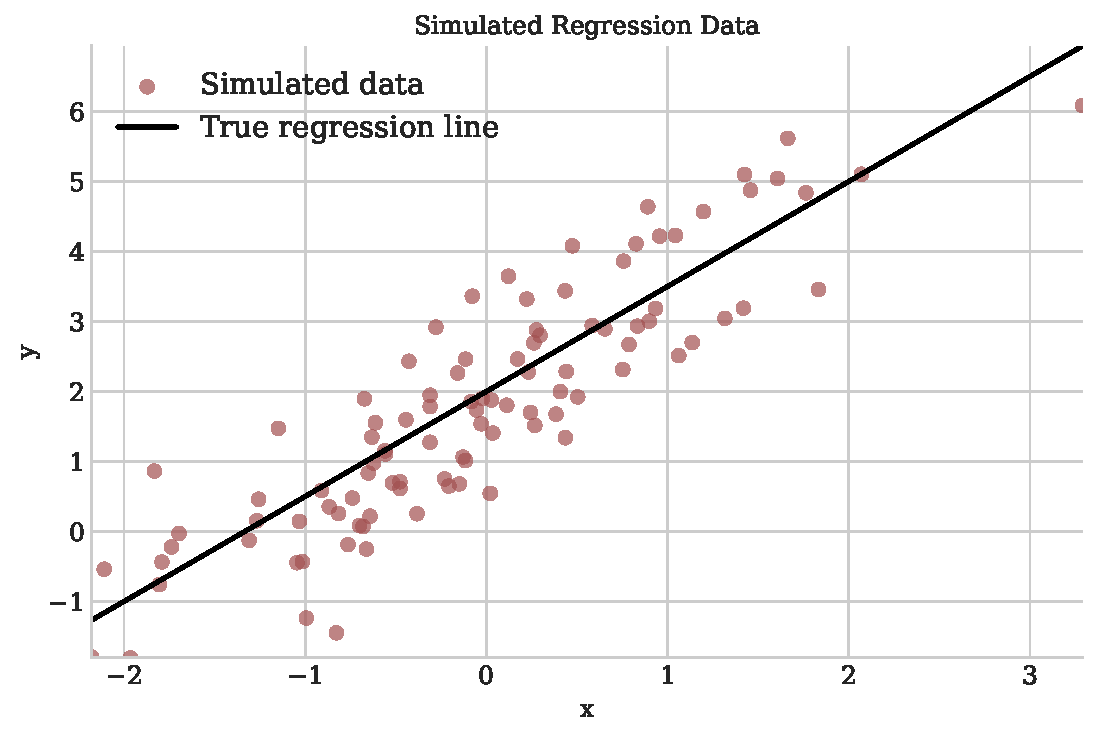
\includegraphics[keepaspectratio]{transforms_files/figure-pdf/cell-3-output-2.pdf}}

In statistics and maths, we have various constraints on some parameters
values. Variances or standard deviations must be positive, probabilities
must be between 0 and 1, correlation matrices must have eigenvalues in
valid ranges, etc. Some of them we know are constrained to be positive
because they are so defined like the standard deviation. Other times, we
know, if these parameters are being intepreted or are structured in some
way, that these parameters must be positive. Assume we don't already
know what our regression parameters values are, as we usually don't. But
we have some idea that they are positive because maybe the intercept
stands for average height and there are no negative height values so no
negative mean heights. This is a constraint imposed by the problem we're
studying.

In Stan, we specify constraints in various ways (see the
\href{https://mc-stan.org/docs/reference-manual/types.html\#variable-declaration.section}{variables
declaration} section for the syntax specification) but typically you'll
see \textless{}``lower=0''\textgreater{} following the function argument
type. This expresses a constraint of positivity on whatever parameter it
attaches to. Here's a Stan model used to fit our simulated data that
uses it for all parameter delcarations.

\begin{codelisting}

\caption{\texttt{model1.stan}}

\begin{Shaded}
\begin{Highlighting}[]
\KeywordTok{data}\NormalTok{ \{}
    \DataTypeTok{int}\NormalTok{\textless{}}\KeywordTok{lower}\NormalTok{=}\DecValTok{0}\NormalTok{\textgreater{} N;}
    \DataTypeTok{vector}\NormalTok{[N] x;}
    \DataTypeTok{vector}\NormalTok{[N] y;}
\NormalTok{\}}

\KeywordTok{parameters}\NormalTok{ \{}
    \DataTypeTok{real}\NormalTok{\textless{}}\KeywordTok{lower}\NormalTok{=}\DecValTok{0}\NormalTok{\textgreater{} alpha;}
    \DataTypeTok{real}\NormalTok{\textless{}}\KeywordTok{lower}\NormalTok{=}\DecValTok{0}\NormalTok{\textgreater{} beta;}
    \DataTypeTok{real}\NormalTok{\textless{}}\KeywordTok{lower}\NormalTok{=}\DecValTok{0}\NormalTok{\textgreater{} sigma; }
\NormalTok{\}}

\KeywordTok{model}\NormalTok{ \{}
\NormalTok{    y \textasciitilde{} normal(alpha + beta * x, sigma);  }
\NormalTok{\}}
\end{Highlighting}
\end{Shaded}

\end{codelisting}

Now, it's quite opaque what exactly the constraints are doing here when
the computation occurs, but we can explictly represent the constraints
Stan computes using the simple transformations Stan is using under the
hood. Here is the model without the constraint syntax but constrained by
explicit syntactic representation of the computation and by updating the
log probability manually.

\begin{codelisting}

\caption{\texttt{model1\_explicit.stan}}

\begin{Shaded}
\begin{Highlighting}[]
\KeywordTok{data}\NormalTok{ \{}
    \DataTypeTok{int}\NormalTok{\textless{}}\KeywordTok{lower}\NormalTok{=}\DecValTok{0}\NormalTok{\textgreater{} N;}
    \DataTypeTok{vector}\NormalTok{[N] x;}
    \DataTypeTok{vector}\NormalTok{[N] y;}
\NormalTok{\}}

\KeywordTok{parameters}\NormalTok{ \{}
    \DataTypeTok{real}\NormalTok{ alpha\_unc; }
    \DataTypeTok{real}\NormalTok{ beta\_unc;}
    \DataTypeTok{real}\NormalTok{ sigma\_unc;}
\NormalTok{\}}

\KeywordTok{transformed parameters}\NormalTok{ \{}
    \DataTypeTok{real}\NormalTok{ alpha = exp(alpha\_unc); }
    \DataTypeTok{real}\NormalTok{ beta = exp(beta\_unc);   }
    \DataTypeTok{real}\NormalTok{ sigma = exp(sigma\_unc); }
\NormalTok{\}}

\KeywordTok{model}\NormalTok{ \{}
    \KeywordTok{target +=}\NormalTok{ alpha\_unc;  }
    \KeywordTok{target +=}\NormalTok{ beta\_unc;  }
    \KeywordTok{target +=}\NormalTok{ sigma\_unc;  }
    
\NormalTok{    y \textasciitilde{} normal(alpha + beta * x, sigma);}
\NormalTok{\}}
\end{Highlighting}
\end{Shaded}

\end{codelisting}

We fit both our models and look at the output summary now.

\begin{Shaded}
\begin{Highlighting}[]
\NormalTok{data }\OperatorTok{=}\NormalTok{ \{}
    \StringTok{\textquotesingle{}N\textquotesingle{}}\NormalTok{: n,}
    \StringTok{\textquotesingle{}x\textquotesingle{}}\NormalTok{: x.tolist(),}
    \StringTok{\textquotesingle{}y\textquotesingle{}}\NormalTok{: y.tolist(),}
\NormalTok{\}}
\end{Highlighting}
\end{Shaded}

\begin{Shaded}
\begin{Highlighting}[]
\NormalTok{model1 }\OperatorTok{=}\NormalTok{ CmdStanModel(stan\_file}\OperatorTok{=}\StringTok{\textquotesingle{}models/model1.stan\textquotesingle{}}\NormalTok{)}
\NormalTok{fit1 }\OperatorTok{=}\NormalTok{ model1.sample(data}\OperatorTok{=}\NormalTok{data, chains}\OperatorTok{=}\DecValTok{4}\NormalTok{, iter\_sampling}\OperatorTok{=}\DecValTok{1000}\NormalTok{, iter\_warmup}\OperatorTok{=}\DecValTok{500}\NormalTok{, show\_progress}\OperatorTok{=}\VariableTok{False}\NormalTok{)}

\NormalTok{fit1.summary()}
\end{Highlighting}
\end{Shaded}

\begin{longtable}[]{@{}lllllllllll@{}}
\toprule\noalign{}
& Mean & MCSE & StdDev & MAD & 5\% & 50\% & 95\% & ESS\_bulk & ESS\_tail
& R\_hat \\
\midrule\noalign{}
\endhead
\bottomrule\noalign{}
\endlastfoot
lp\_\_ & -27.622300 & 0.027799 & 1.214040 & 1.002390 & -30.073900 &
-27.317500 & -26.280500 & 1976.00 & 2405.99 & 1.00268 \\
alpha & 1.877840 & 0.001274 & 0.081531 & 0.080550 & 1.743550 & 1.877650
& 2.012280 & 4108.88 & 2843.57 & 1.00119 \\
beta & 1.525980 & 0.001304 & 0.081460 & 0.082344 & 1.392380 & 1.524590 &
1.661810 & 3924.87 & 2613.48 & 1.00351 \\
sigma & 0.809912 & 0.001003 & 0.059192 & 0.056371 & 0.718451 & 0.806936
& 0.912513 & 3579.25 & 2652.97 & 1.00011 \\
\end{longtable}

\begin{Shaded}
\begin{Highlighting}[]
\NormalTok{model1\_explicit }\OperatorTok{=}\NormalTok{ CmdStanModel(stan\_file}\OperatorTok{=}\StringTok{\textquotesingle{}models//model1\_explicit.stan\textquotesingle{}}\NormalTok{)}
\NormalTok{fit2 }\OperatorTok{=}\NormalTok{ model1\_explicit.sample(data}\OperatorTok{=}\NormalTok{data, chains}\OperatorTok{=}\DecValTok{4}\NormalTok{, iter\_sampling}\OperatorTok{=}\DecValTok{1000}\NormalTok{, iter\_warmup}\OperatorTok{=}\DecValTok{500}\NormalTok{, show\_progress}\OperatorTok{=}\VariableTok{False}\NormalTok{)}

\NormalTok{fit2.summary()}
\end{Highlighting}
\end{Shaded}

\begin{longtable}[]{@{}lllllllllll@{}}
\toprule\noalign{}
& Mean & MCSE & StdDev & MAD & 5\% & 50\% & 95\% & ESS\_bulk & ESS\_tail
& R\_hat \\
\midrule\noalign{}
\endhead
\bottomrule\noalign{}
\endlastfoot
lp\_\_ & -27.566200 & 0.027273 & 1.182140 & 0.968434 & -29.892600 &
-27.255300 & -26.265100 & 2050.02 & 2289.04 & 1.00077 \\
alpha\_unc & 0.629589 & 0.000655 & 0.041943 & 0.041334 & 0.559548 &
0.631160 & 0.697422 & 4156.59 & 2745.01 & 1.00059 \\
beta\_unc & 0.420922 & 0.000804 & 0.052845 & 0.053089 & 0.331678 &
0.423594 & 0.505266 & 4369.39 & 3162.81 & 0.99954 \\
sigma\_unc & -0.210302 & 0.001363 & 0.071842 & 0.070495 & -0.323411 &
-0.212575 & -0.088289 & 2813.00 & 2354.88 & 1.00071 \\
alpha & 1.878490 & 0.001227 & 0.078695 & 0.077755 & 1.749880 & 1.879790
& 2.008570 & 4156.60 & 2745.01 & 1.00059 \\
beta & 1.525490 & 0.001216 & 0.080304 & 0.081024 & 1.393310 & 1.527440 &
1.657430 & 4369.41 & 3162.81 & 0.99954 \\
sigma & 0.812439 & 0.001120 & 0.058713 & 0.057120 & 0.723676 & 0.808500
& 0.915497 & 2813.03 & 2354.88 & 1.00075 \\
\end{longtable}

We see the two Stan models provided are mathematically equivalent and
will recover the same parameter values because they involve two closely
identical computations of the same reparameterization, a constrain of
positivity. The key difference between them lies in where the code is
being represented. Stan does it somewhere else as a subroutine not
represented to the user, but we did it directly. We'll break the math
down in a bit more detail now.

In the first model, the parameters \(\alpha\), \(\beta\), \(\sigma\) are
constrained to be greater than or equal to 0 (i.e., \(\alpha\),
\(\beta\), and \(\sigma\) \(\geq\) \(0\)). This means the model
explicitly ensures these parameters are non-negative during sampling.

Stan will sample these parameters directly in their constrained space
(keep in mind: sampling in the constrained space is NOT equivalent to
sampling and transforming your sample to be constrained. We'll revisit
this below). The parameter values are bounded between \(0\) and
\(\infty\). This means the likelihood will incorporate the probability
of the parameters being within the defined range, i.e., using the normal
distribution for the regression model, along with the boundary
conditions on the parameters (such as \(\sigma \geq 0\) ).

Both models are mathematically\footnote{Not computationally equivalent.
  Besides that point, it's also not true that a change of variables
  preserves the log density. It would defeat the purpose if it did,
  since the transformation defines a probability density, which is a
  non-unique, parameterization-dependent function in
  \(\mathbb{R}^N \to \mathbb{R}_+\). In practice, this means a given
  model can be represented different ways, and different representations
  have different computational performances. There are at least two
  levels of representation of a model going on here. One is at the low
  level (where we are) where we have changes in the log density due to
  various computations performed on it. The other level is one we'll get
  to in the next section where we reparameterize a model by composing it
  with some functions to transform the sampled outputs. This is what you
  typically do, for example, in reparameterizing a beta distribution
  with the mean and total counts rather than in terms of the two counts,
  \(\alpha\) and \(\beta\). This reparameterization doesn't distort the
  underlying log density when you sample because it's done after the
  fact.} equivalent because the transformations in the second model
enforce the same constraints on the parameters as the first model but
instead of performing the adjustment on the log density automatically as
Stan does if you specify bounds, we do it by hand (Why increment the
target probability by the value \(X_{unc}\) you might ask? Keep
reading). The transformation \(\exp(x)\) maps all real values of
\(\alpha_{\text{unc}}\), \(\beta_{\text{unc}}\), and
\(\sigma_{\text{unc}}\) to positive values, which is what the first
model does by directly imposing constraints
\(\alpha, \beta, \sigma \geq 0\).

\begin{itemize}
\tightlist
\item
  In the first model, the parameter space is constrained to be
  non-negative directly, so Stan only samples within the range
  \([0, \infty]\).
\item
  In the second model, the parameters are unconstrained, and the
  exponential transformation ensures that the resulting parameters are
  positive. The log of the Jacobian
  \(\log \left( \left| \frac{d}{dx} \exp(x) \right| \right)\) is then
  added to the target log-probability to adjust for the transformation
  from unconstrained space to constrained space because we want to
  interpret our sampling in the original space.
\end{itemize}

Both methods perform close to identical operations\footnote{Not exactly.
  \href{https://mc-stan.org/docs/reference-manual/transforms.html\#lower-bound-transform.section}{Stan
  uses the general transformation} \(X = \exp(Y) + a\) for a lower bound
  constraint being \(a\).} for the log densities and will therefore
produce the same parameter values after sampling. This is because both
models are doing the same reparameterization.

More precisely, the likelihood function in both models is:

\[
y_i \sim \mathcal{N}(\alpha + \beta x_i, \sigma)
\]

In the second model, the unconstrained parameters
\(\alpha_{\text{unc}}, \beta_{\text{unc}}, \sigma_{\text{unc}}\) are
mapped to positive values via the exponential function:

\[
\alpha = \exp(\alpha_{\text{unc}}), \quad \beta = \exp(\beta_{\text{unc}}), \quad \sigma = \exp(\sigma_{\text{unc}})
\]

The Jacobian of this transformation is:

\[
\frac{d}{d\theta} \exp(\theta) = \exp(\theta)
\]

So, the log-Jacobian adjustment is:

\[
\log(\exp(\alpha_{\text{unc}})) = \alpha_{\text{unc}}, \quad \log(\exp(\beta_{\text{unc}})) = \beta_{\text{unc}}, \quad \log(\exp(\sigma_{\text{unc}})) = \sigma_{\text{unc}}
\]

Thus, the log-probability is adjusted by adding these terms to account
for the transformation from the unconstrained space to the constrained
space. Stan typically does these change of variable transformations
automatically using a more generalized transformation for the
lower-bound constraint. But I find it quite nice that Stan allows you to
program things manually and increment the log density using target+=.
You might ask why would I ever care to figure out what the log Jacobian
adjustment is when Stan can do it for me?\footnote{Besides the fact that
  it's nice to know you can do it and you should know what Stan is
  doing!} You don't ever need to if all you're doing is specifying
constraints like the ones Stan provides for variables, but there are
constraints that you would want to impose that do require it. There are
too many reasons you'd want to that I'm unaware of but here are a few:
high posterior correlation in unconstrained space (cf.~Neal's funnel),
numerical stability, prior stability, and sampling efficiency. It would
take too long to go into the details and Google is your best friend
here. Outside of Bayesian inference related things, constrained
transformation have found a home in some kick ass generative models that
are based on Normalizing Flows.\footnote{Again Google.}

Looking back at our models you might wonder if these non-linear
transformation applied are actually changing the underlying density
substanitally. You'd be right to think this. For our example, we can
refit the model without the Jacobian adjustment and see what happens.

\begin{codelisting}

\caption{\texttt{model1\_explicit.stan}}

\begin{Shaded}
\begin{Highlighting}[]
\KeywordTok{data}\NormalTok{ \{}
    \DataTypeTok{int}\NormalTok{\textless{}}\KeywordTok{lower}\NormalTok{=}\DecValTok{0}\NormalTok{\textgreater{} N;}
    \DataTypeTok{vector}\NormalTok{[N] x;}
    \DataTypeTok{vector}\NormalTok{[N] y;}
\NormalTok{\}}

\KeywordTok{parameters}\NormalTok{ \{}
    \DataTypeTok{real}\NormalTok{ alpha\_unc; }
    \DataTypeTok{real}\NormalTok{ beta\_unc;}
    \DataTypeTok{real}\NormalTok{ sigma\_unc;}
\NormalTok{\}}

\KeywordTok{transformed parameters}\NormalTok{ \{}
    \DataTypeTok{real}\NormalTok{ alpha = exp(alpha\_unc); }
    \DataTypeTok{real}\NormalTok{ beta = exp(beta\_unc);   }
    \DataTypeTok{real}\NormalTok{ sigma = exp(sigma\_unc); }
\NormalTok{\}}

\KeywordTok{model}\NormalTok{ \{}
\NormalTok{    y \textasciitilde{} normal(alpha + beta * x, sigma);}
\NormalTok{\}}
\end{Highlighting}
\end{Shaded}

\end{codelisting}

\begin{Shaded}
\begin{Highlighting}[]
\NormalTok{model1\_explicit\_no\_increment }\OperatorTok{=}\NormalTok{ CmdStanModel(stan\_file}\OperatorTok{=}\StringTok{\textquotesingle{}models//model1\_explicit\_no\_increment.stan\textquotesingle{}}\NormalTok{)}
\NormalTok{fit3 }\OperatorTok{=}\NormalTok{ model1\_explicit\_no\_increment.sample(data}\OperatorTok{=}\NormalTok{data, chains}\OperatorTok{=}\DecValTok{4}\NormalTok{, iter\_sampling}\OperatorTok{=}\DecValTok{1000}\NormalTok{, iter\_warmup}\OperatorTok{=}\DecValTok{500}\NormalTok{, show\_progress}\OperatorTok{=}\VariableTok{False}\NormalTok{)}

\NormalTok{fit3.summary()}
\end{Highlighting}
\end{Shaded}

\begin{longtable}[]{@{}lllllllllll@{}}
\toprule\noalign{}
& Mean & MCSE & StdDev & MAD & 5\% & 50\% & 95\% & ESS\_bulk & ESS\_tail
& R\_hat \\
\midrule\noalign{}
\endhead
\bottomrule\noalign{}
\endlastfoot
lp\_\_ & -28.465300 & 0.027567 & 1.255610 & 1.004020 & -30.902100 &
-28.137100 & -27.114300 & 2184.55 & 2489.87 & 1.000710 \\
alpha\_unc & 0.628232 & 0.000724 & 0.044194 & 0.044910 & 0.555909 &
0.628785 & 0.699591 & 3742.07 & 3012.52 & 1.000300 \\
beta\_unc & 0.417134 & 0.000811 & 0.054371 & 0.054282 & 0.326635 &
0.417550 & 0.504227 & 4536.13 & 3117.52 & 1.001010 \\
sigma\_unc & -0.213706 & 0.001194 & 0.070709 & 0.070322 & -0.326706 &
-0.215641 & -0.094641 & 3567.97 & 2934.72 & 0.999307 \\
alpha & 1.876120 & 0.001359 & 0.082917 & 0.084278 & 1.743530 & 1.875330
& 2.012930 & 3742.04 & 3012.52 & 1.000260 \\
beta & 1.519840 & 0.001227 & 0.082412 & 0.082573 & 1.386290 & 1.518240 &
1.655700 & 4536.21 & 3117.52 & 1.000910 \\
sigma & 0.809614 & 0.000980 & 0.057637 & 0.056042 & 0.721296 & 0.806024
& 0.909699 & 3567.97 & 2934.72 & 0.999291 \\
\end{longtable}

Nothing seems to have changed except a decrease in the log probability.
The underlying density doesn't exactly match anymore. But, this doesn't
mean our inference goes totally awary. The parameters estimates match
our first two model estimates because the underlying geometry wasn't
distorted by much. We shouldn't expect it to for a simple model where
the data is fairly well behaved. We're also not applying the
transformation on our observed output value \(y\) to expect much of a
change, and the likelihood term isn't affected as much by the
transformations of the parameters because we have enough data for the
estimation to find the posterior mean easily. Even if we had
substantially less data in our case we would still be able to find it
because we're conducting a simple transformation on parameters we know
are positive.

\section{A Note on Change of Variables VS.
Transformations}\label{a-note-on-change-of-variables-vs.-transformations}

Smarter people than I have tried to drill this distinction down. I
highly, highly recommend reading and rereading the Stan documentation
\href{https://mc-stan.org/docs/stan-users-guide/reparameterization.html\#change-of-variables.chapter}{here}.
They give many examples at varying complexity and really hammer home the
difference.

To put it succietnly, change of variables transformation are
transformations that first transform the variables AND THEN sample them.
Whereas transformations are typically taken to be instances where we
sample some variables AND THEN apply a functional transformation to
them. Again, read that Stan article. It provides many examples that
demonstrate the difference.

Before moving onto the architecture for our own transform class, I'll
plug in two nice articles. One of them by
\href{https://jsocolar.github.io/jacobians/\#fn9}{Jacob Socolar}
clarifies the nature of the Jacobian adjustment with a simple example.
He links to various soruces on the same topic in there that are well
worth a look. The other post is by
\href{https://users.aalto.fi/~ave/casestudies/Jacobian/jacobian.html}{Aki
Vehtari} and gives a nice treatment of the Laplace approximation and
Jacobian adjustment, going slighly more in depth. I said two but I can't
leave out
\href{https://betanalpha.github.io/assets/case_studies/probability_theory.html\#4_representing_probability_distributions_with_densities}{this}
article by Michael Betancourt that does go through the mathematical
details in the section linked. Socolar links to it and \emph{highly
recommends} it. As do I. Betancourt's work is always
top-tier.\footnote{LOVE his work. Best stuff out there! Read it and buy
  him a coffee \href{https://www.patreon.com/betanalpha}{here} if you
  feel you got something out of it.}

\section{Some Quick Mathematics for Probability and Constrained
Transformations}\label{some-quick-mathematics-for-probability-and-constrained-transformations}

``It would be good to cover the foundations of continous probability
theory. Start with a space consisting of an ambient set \(X\), endowed
with a \(\sigma\)-algebra \(\mathcal{X}\) consisting of all well-behaved
subsets of \(X\) and a probability distribution \(\pi\) that maps
elemens of the \(\sigma\)-algebra into probabilities in a way that's
comptabile with countable unions, intersections, and
complements.''\footnote{\href{https://discourse.mc-stan.org/t/why-transformations-need-to-be-invertible-in-change-of-variable-in-probability-theory/22317/11?u=mike1}{Betancourt}}

When working with probability theory, particulary on \(\mathbb{R}^n\),
the choice of \(\sigma\)-algebra is crucial. The two most common
\(\sigma\)-algebras are (1) Borel \(\sigma\)-algebra,
\(\mathcal{B}(\mathbb{R}^n)\), generated by all open sets in
\(\mathbb{R}^n\). These include intervals, rectangles, and their
countable operations. And (2) Lebesgue \(\sigma\)-algebra,
\(\mathcal{L}(\mathbb{R}^n)\), which are an extension of the Borel
\(\sigma\)-algebra that includes more sets. The relationship between
these is:

\[
\mathcal{B}(\mathbb{R}^n) \subset \mathcal{L}(\mathbb{R}^n)
\]

\(\mathcal{L}(\mathbb{R}^n)\) contains all Borel sets plus all subsets
of Borel sets with Lebesgue measure zero. When considering
transformations between spaces, these distinctions become important:
measurable functions must preserve the \(\sigma\)-algebra structure.

``When considering another space \(Y\) equipped with its own
\(\sigma\)-algebra \(\mathcal{Y}\) along with a map
\(F: X \rightarrow Y\), this point-wise mapping can induce maps between
objects defined on these spaces. The original map \(F\) induces both a
pushforward map (in the same direction of \(F\)) and a pullback map (in
the opposite direction of \(F\)) between subsets on \(X\) and \(Y\). If
the pullback map is compatible with the \(\sigma\)-algebras so that for
every \(B \in \mathcal{Y}\) we have \(F^{-1}(B) \subset \mathcal{X}\),
then we can define an induced pushforward map between probability
distributions. Every probability distribution \(\pi\) defined on \(X\)
defines a pushforward probability distribution \(F_\pi\) on \(Y\) via
\(P_{F_\pi}[B] = P_\pi[F^{-1}(B)]\).

Now let's consider another space \(Y\) equipped with its own
\(\sigma\)-algebra \(\mathcal{Y}\) along with a map
\(F: X \rightarrow Y\).

Nominally \(F\) just maps points in \(X\) to points in \(Y\) but this
point-wise mapping can also induce maps from objects defined on \(X\) to
objects defined on \(Y\). For example by breaking a subset
\(A \subset X\) into points and then mapping them to \(Y\) before
collecting those output points in other subset \(F(A) \subset Y\) the
original map \(F\) induces a map from subsets on \(X\) to subsets on
\(Y\). This kind of induced map in the same direction of \(F\) is called
a \emph{pushforward} along \(F\).

At the same time \(F\) might also induce maps from objects defined on
\(Y\) to objects defined on \(X\). If \(F\) isn't bijective then we
can't define an inverse point-wise map \(F^{-1} : Y \rightarrow X\), but
we can we can define a map from subsets \(B \subset Y\) to subsets
\(F^{-1}(B) \subset X\). This kind of induced map in the opposite
direction of \(F\) is called a \emph{pullback} along \(F\).

So the point-wise map \(F\) induces both a pushforward and pullback map
between subsets on \(X\) and \(Y\). These induced maps, however, will
not in general respect the \(\sigma\)-algebras. In particular if
\(A \in \mathcal{X}\) then the output of the pushforward map \(F(A)\)
need not be in \(\mathcal{Y}\), and vice versa for the pullback map.

If the pullback map is compatible with the \(\sigma\)-algebras so that
for every \(B \in \mathcal{Y}\) we have
\(F^{-1}(B) \subset \mathcal{X}\) then we can define \emph{another}
induced pushforward map, this time between probability distributions.
Every probability distribution \(\pi\) defined on \(X\) defines a
pushforward probability distribution \(F_{*} \pi\) on \(Y\) via the
probabilities

\[
\mathbb{P}_{F_{*} \pi}[B] = \mathbb{P}_{\pi}[ F^{-1}(B) ].
\]

Again we need \(F^{-1}(B)\) to be in \(\mathcal{X}\) otherwise the
initial probability distribution won't know how to assign a probability
to the pullback subset.

\emph{Measurable} functions/maps/transformations are just the maps
satisfying the compatibility requirement that allows us to define
pushforward probability distributions. In other words measurable maps
are the only maps that allow us to translate probability distributions
from one space to another.

Note that at this point no other requirement has been made on the
structure of \(X\), \(Y\), and \(F\). \(X\) and \(Y\) don't have to have
the same dimensions, \(F\) doesn't have to be bijective or even
injective so long as it satisfies the \(\sigma\)-algebra consistency
property.

If the dimension of \(Y\) is less than the dimension of \(X\) then a
measurable surjection \(F : X \rightarrow Y\) is commonly known as
projection map, and pushforward distributions are known as
\emph{marginal} distributions.

If the dimension of \(X\) and \(Y\) are the same and both \(F\) and
\(F^{-1}\) are measurable then a bijection \(F: X \rightarrow Y\) is
commonly known as a reparameterization.

(Side note: codomains are irrelevant here as the \(\sigma\)-algebras and
probability distributions of interest are all defined over the entire
domain).

They key difference between these two types of maps is that projections
loose information while reparameterizations do not. If \(F\) is a
reparameterization then we can start at \(\pi\) on \(X\), pushforward to
\(F_{*} \pi\) on \(Y\), then pushforward along \(F^{-1}\) to recover the
original distribution,

\[
(F^{-1})_{*} F_{*} \pi = \pi.
\]

This is not true of projection functions -- we can map \(\pi\) on \(X\)
to \(F_{*} \pi\) on \(Y\) but there's no way to recover \(\pi\) from
that pushforward distribution.

Okay, so now we're \emph{finally} ready to talk about probability
density functions. Probability density functions are functions that
quantify the difference between two measures. Mathematically we denote
the density function of \(\pi_{2}\) with respect to \(\pi_{1}\) as

\[
\pi_{21}(x) = \frac{ \mathrm{d} \pi_{2} }{ \mathrm{d} \pi_{1} } (x).
\]

Most often we correct some standard ``uniform'' distribution on the
ambient space to the probability distribution of interest. If \(X\) is a
real space then that uniform distribution is the Lebesgue measure,
\(\mathcal{L}\). In other words the probability density function of
\(\pi\) is actually the probability density function of \(\pi\) relative
to the Lebesgue measure,

\[
\pi(x) = \frac{ \mathrm{d} \pi }{ \mathrm{d} \mathcal{L} } (x).
\]

Using the above machinery we can in some cases work out how to construct
pushforward probability density functions. The basic idea is to take a
distribution on \(X\), push it forward along \(F\) to \(F_{*} \pi\) on
\(Y\) and then construct the density of each with respect to the uniform
measures on \(X\) and \(Y\) respectively. In other words

\[
\pi(x) = \frac{ \mathrm{d} \pi }{ \mathrm{d} \mathcal{L}_{X} } (x) \mapsto \pi(y) = \frac{ \mathrm{d} F_{*} \pi }{ \mathrm{d} \mathcal{L}_{Y} } (y).
\]

Notice that we pushforward \(\pi\) along \(F\) but we define the
densities with respect to the uniform distributions on \(X\) and \(Y\)
respectively. We don't transform the uniform distribution on \(X\) to
some distribution on \(Y\) because that pushforward distribution will in
general no longer be uniform! Indeed when \(F: X \rightarrow Y\) is a
measurable bijection the amount by which \(F\) warps the initial uniform
distribution is just the Jacobian determinant!

Mathematically when \(F\) is a bijection we can write

\[
\pi(y) = \frac{ \mathrm{d} F_{*} \pi }{ \mathrm{d} \mathcal{L}_{Y} } (y) = \frac{ \mathrm{d} F_{*} \pi }{ \mathrm{d} F_{*} \mathcal{L}_{X} } (y) \cdot \frac{ \mathrm{d} F_{*} \mathcal{L}_{X} }{ \mathrm{d} \mathcal{L}_{Y} } (y) = \pi(F^{-1}(y)) \cdot | J |(y)
\]

which is exactly the usual ``change of variables'' formula that's pulled
out of thin air.

When \(F\) is a surjection then the density of the pushforward uniform
distribution from \(X\) relative to the uniform distribution on \(Y\),
\(\mathrm{d}\mathcal{L}_{X}\)/\(\mathrm{d}\mathcal{L}_{Y}\) is singular
and so the usual change of variables formula cannot be applied. In these
cases working out the pushforward probability density functions, or the
marginal density functions, is much, much harder and usually cannot be
done analytically.''\footnote{\href{https://discourse.mc-stan.org/t/why-transformations-need-to-be-invertible-in-change-of-variable-in-probability-theory/22317/11?u=mike1}{Betancourt}}

\section{Contraint Transformations in
GPJaxStuff}\label{contraint-transformations-in-gpjaxstuff}

Why should we care about contraint transformations for Gaussian
Processes? We can enforce various kinds of contraints on our mean
function, kernel outputs, kernel parameters, or predictions. GPs are
glorified priors on function spaces. We should be constraining that
space as much as possible. The structure of our




\end{document}
